\documentclass[
  11pt,					% Schriftgröße
  paper=a4,
  DIV=13,				% Seitenlayout (Satzspiegel)
  parskip=half,			% Abstand zwischen Absätzen
  %twoside,				% Doppelseitig
  openright,			% neues Kapitel rechts
%  cleardoublepage,
  bibtotoc,				% Literaturverzeichis in Inhaltsverzeichnis
  headsepline,			% Kopfzeilentrennlinie
  headings,	
%  draft,				% Korrekturfassung
  ]{scrreprt}		% scrartcl	

% Algorithmen
\usepackage{algorithm}
\usepackage{algpseudocode}

% Eingabecodierung
\usepackage[utf8]{inputenc}

% Schriftcodierung
\usepackage[T1]{fontenc}

% Sprachraum
\usepackage[ngerman]{babel}

% Blindtext
\usepackage{blindtext}
 
% Schrifteinstellungen
\usepackage{lmodern} 		% Vektorschrift
\renewcommand{\familydefault}{\sfdefault} % Serifenlose Schrift
\usepackage{sansmath}  	% Mathe-Schrift ohne Serifen
%\sansmath 							% aktiviert serifenlose Matheschrift
\usepackage{microtype}	% harmonische Typenverteilung

% Literatur einbinden
\usepackage{csquotes}	% Steuerung der Anführungszeichen
\usepackage[
  backend=biber,			% Sortier-Compiler
  style=numeric-comp,	% Zitationsstil
  block=ragged,
  ]{biblatex}

\addbibresource{ref/ref_liste.bib}

% Mathemodus
\usepackage{amsmath,amssymb}

% Trennung
\hyphenation{Crash-zo-ne}

% Bilder einbinden
\usepackage{graphicx}
\graphicspath{{bilder/}}
\usepackage{svg}

% Kopf- und Fußzeile
\usepackage[
	headsepline,	% Kopfzeilen-Sepparationslinie
	automark,		% Lebende Kolumnentitel
	]
	{scrlayer-scrpage}
\pagestyle{scrheadings}		
\ofoot*{\pagemark}			
\ohead{\headmark}

% Codebeispiele
\usepackage{minted}

% Titelseite



\titlehead{
		\hfil
		  
\includegraphics[width=0.3\textwidth]{thi_logo}
		  \hfil
  }


\title{\vspace{5ex} Roboternavigation mit Potenzialfeldern}

\subtitle{ \vspace{6ex} \Large Intelligente Robotik WS2023/24\\Praktische Arbeit \vspace{5ex}}

\author{Carl Schünemann (Mat.Nr. $00107827$)}

\date{\today}
  

\begin{document}
  
  % Titelseite anzeigen
  \maketitle
  
  \pagenumbering{Roman}

  
  % Inhaltsverzeichnis
  \tableofcontents
  
  \cleardoubleoddpage
  \pagenumbering{arabic}

  
  % Kapitel einbinden
  \chapter{Ziel der Implementierung}

Die vorliegende Arbeit dokumentiert die praktische Umsetzung eines Planungssystems zur Roboternavigation im Rahmen der Vorlesung ``Intelligente Robotik`` im Wintersemester 2023/24 an der THI.

Die Implementierung erfolgte in Python, wobei ein Jupyter Notebook als zentraler Einstiegspunkt dient. 
Ein rechteckiger Roboter variabler Größe navigiert in einem statisch vorgegebenen Occupancy Grid mit beliebig konfigurierbaren Hindernissen von einem Start- zum Zielpunkt.
Die kollisionsfreie Roboternavigation wird durch die Transformation der Roboterbewegung in einen dreidimensionalen Konfigurationsraum nach einem Ansatz von Yunfeng und Chirikjian ermöglicht \cite{wang.2000}.
Die Routenplanung von Start- zu Zielpunkt basiert auf Potenzialfeldern, deren Berechnung sowohl mit anziehenden und abstoßenden Potenzialen als auch dem Wavefront-Algorithmus implementiert wurde. 
Die Roboternavigation erfolgt durch das Gradientenabstiegsverfahren in den Kraftfeldern der Potenzialfelder. 
Diverse grafische Darstellungen visualisieren die Berechnungen und Roboternavigation.

Nachfolgendes Kapitel dient als Kurzanleitung zur Ausführung des Programms. Die weiteren Kapitel befassen sich mit dem theoretischen Hintergrund der Implementierung.

%Nachfolgende Arbeit dient der Dokumentation der Praktischen Arbeit für die Vorlesung "Intelligente Robotik" im Wintersemster 2023/24.
%- Planungssystem zur Roboternavigation 
%- Umgesetzt in Python. Zentraler Einstiegspunkt: Jupyter Notebook
%- Rechteckiger Roboter mit Variabler Größe (width, length)
%- Translation und Rotation in einem statisch gegebenem Occupancy Grid mit beliebig konfigurierbaren Hindernissen für verschiedene Planungsszenarien.
%- Kollisionsfreie Roboternavigation durch Transformation der Roboterbewegung in dreidimensionalen Konfiguraionsraum gemäß dem Ansatz von XYZ (TODO!).
%- Roboternavigation von Start- zu Zielpunkt basierend auf Potenzialfeldern: In Implementierung sowohl Berechnung mit anziehendem und abstoßendem Potenzialen realisiert als auch über den Wavefront-Algorithmus 
%- Roboternavigation durch Gradientenabstiegsverfahren in Kraftfeldern der Potenzialfelder.
%- Visualisierung der Berechnungen und der Roboternavigation.
%
%Aufbau Arbeit:
%- Nachfolgendes Kapitel = Kurzanleitung zur Ausführung
%- Alle darauf folgenden restlichen Kapitel befassen sich mit dem theoretischen Hintergrund der Implementierung

  % Kapitel einbinden
  \chapter{Technische Voraussetzungen}

- Implementierung in Python mit einem Jupyter Notebook. 
- Quellcode auf GitHub: (QR-Code)

- Bedingungen zur Ausführung: Python >= 3.7
- Python Abhängigkeiten:
	> matplotlib zur Visualisierung
	> numpny für Mathematische Berechnungen
	=> Installation aller Abhängigkeiten: pip install -r requirements.txt

- Empfehlung zur Ausführung: Anacoda Environment

  % Kapitel einbinden
  \chapter{Robotermodell}
  
  % Kapitel einbinden
  \chapter{Konfigurationsraum}

Roboter befindet sich in "Occupancy-Grid": 2D Boolean Array "occupancy-grid" der Größe "occu-size-y" x "occu-size-x", das der Umgebung des Roboters entspricht, mit Ursprung "links oben"
Für ein Hindernis an der Stelle (X,Y) steht im Occupancy-Grid "False", für eine freie Koordinate "True"

Translation: "x-1" (links), "x+1" (rechts), "y-1" (oben), "y+1" (unten)

*** TODO: Abbildung 2D Occupancy Grid ***

Umsetzung der Kombination aus variabler Größe + Roboterrotation: Ansatz aus Literatur ... (TODO): 
- Transformation der Bewegung des Roboters der Größe "width", "length" in die Punkt-Bewegung des Roboters mit Größe width=1, length=1
- Deshalb für jede der möglichen 4 Rotationen des Roboters (0°, 90°, 180°, 270°): neues Occupancy-Grid in dem das ursprüngliche Occupancy-Grid um die Roboterdimensionen der jeweiligen Rotation erweitert wurde
=> Ergebnis: 4x 2D-Occupancy-Grids mit erweiterten Hindernis = 4x "Rotationsebene"

*** TODO: Abbildung der erweiterten Occupancy Grids"

=> Zusammenfassen zu einem 3D-Array "configuration-space[rotation][y][x] der Dimension 4 x "occu-size-y" x "occu-size-y"
=> Rotation: in Rotationsbene "rotation": 
	- "(rotation+1) mod 4" (Rotation um 90° im Uhrzeigersinn)
	- "(rotation-1) mod 4" (Rotation um 90° gegen Uhrzeigersinn)

*** TODO: Abbildung 3D Plot ***

3D Konfigurationsraum ermöglicht somit 
	1. kollisionsfreie Translation
	2. kollisionsfreie Rotation


  \chapter{Berechnung der Potenzialfelder}

Die Grundlage der Pfadplanung zu einem Zielpunkt bildet in dieser Implementierung die \textit{Potenzialfeldmethode}:
Der Konfigurationsraum entspricht einem skalaren \textit{Potenzialfeld}, wobei jede Koordinate eine potenzielle Energie $U(\texttt{x}, \texttt{y}, \texttt{rotation})$ besitzt, ausgedrückt durch eine reelle Zahl.
Je Höher die potenzielle Energie einer Koordinate, desto weiter ist der Punkt auf dem aktuellen Pfad vom Ziel entfernt.
Die Berechnung des Potenzialfelds $\texttt{potential[rotation][y][x]} = U(\texttt{x}, \texttt{y}, \texttt{rotation})$ erfolgt mit \textit{Potenzialfunktionen}. \cite{yujiang.2017}

\vspace*{0.2cm}
\section{Anziehende \& abstoßende Potenziale} \label{sec:attr-repul-pot}

Khatib schlug 1986 vor, das Potenzialfeld analog zu Magnet- und Gravitationsfeldern zu berechnen \cite{khatib.1985}. Der zu erreichende Zielpunkt wirkt mit einem \textit{anziehenden} (engl. \textit{attractive}) Potenzial auf eine Koordinate (\texttt{y}, \texttt{x}). Dieses Potenzial ist in allen Rotationsebenen gleich:
\vspace*{0.25cm}
\begin{equation*}
U_{Attr, Ziel}(\texttt{x}, \texttt{y}) = \sqrt{(\texttt{y} - \texttt{y}_{Ziel})^2 + (\texttt{x} - \texttt{x}_{Ziel})^2}
\end{equation*}

%\vspace*{-0.1cm}
Bei den getesteten Implementierungsszenarien wurden bessere Ergebnisse festgestellt, wenn das anziehenden Potenzial erst normiert und anschließend gewichtet wird. Mit $\texttt{attraction\_weight} = 1$ hat das anziehende Potenzial einen Wertebereich von $[0;1]$. Mit  $\texttt{attraction\_weight} < 1$ wird die obere Grenze des Wertebereichs gegen $0$ verringert, mit $\texttt{attraction\_weight} > 1$ wird sie über $1$ vergrößert:
\vspace*{0.3cm}
\begin{equation*}
U_{Attr, Ziel}(\texttt{x}, \texttt{y})_{norm} = \frac{U_{Attr, Ziel}(\texttt{x}, \texttt{y})}{\max \{ U_{Attr, Ziel}\}} * \texttt{attraction\_weight} 
\end{equation*}

%\vspace*{-0.1cm}
Die Hindernisse im Konfigurationsraum wirken auf jede Koordinate (\texttt{x}, \texttt{y}, \texttt{rotation}) mit einem \textit{abstoßendem} (engl. \textit{repulsive}) Potenzial. Das umfasst auch die Hindernisse in den benachbarten Rotationsebenen \texttt{((rotation+1) \% rotations)} sowie \texttt{((rotation-1) \% rotations)}. Mit $\texttt{repulsion\_weight}=0$ hat das abstoßende Potenzial einen Wertebereich von $[0;g]$, wobei $0\le g \le 1$. Werte $\texttt{repulsion\_weight} > 0 $ verringern die obere Grenze des Wertebereichs gegen $0$: \cite{schweiger.2023}
\vspace*{0.25cm}
\begin{equation*}
\hspace*{-0.075\linewidth}
\resizebox{1.15\linewidth}{!}{
  $ U_{Repul, Hindernis}(\texttt{x}, \texttt{y}, \texttt{rotation}) = \frac{1}{\texttt{repulsion\_weight} + \sqrt{(\texttt{y} - \texttt{y}_{Hindernis})^2 + (\texttt{x} - \texttt{x}_{Hindernis})^2 + (\texttt{rotation} - \texttt{rotation}_{Hindernis})^2}}
$}
\hspace*{-0.075\linewidth}
\end{equation*}

\vspace*{0.05cm}
Yujiang und Huilin definieren das abstoßende Potenzial einer Koordinate als kleinsten Abstand zu allen Hindernissen \cite{yujiang.2017}:
\vspace*{0.3cm}
\begin{equation*}
U_{Repul}(\texttt{x}, \texttt{y}, \texttt{rotation}) = \min_{\forall \,\,Hindernis \,\,\in \texttt{ occupancy\_grid}} \{ U_{Repul, Hindernis}(\texttt{x}, \texttt{y}, \texttt{rotation}) \}
\end{equation*}

%\vspace*{-0.1cm}
Die gesamte potenzielle Energie einer Koordinate entspricht der Kombination beider Potenziale. In dieser Implementierung wurden anziehendes und abstoßendes Potenzial gemäß Khalib addiert \cite{khatib.1985}:
\vspace*{0.25cm}
\begin{equation*}
U(\texttt{x}, \texttt{y}, \texttt{rotation}) = U_{Attr, Ziel}(\texttt{x}, \texttt{y})_{norm} + U_{Repul}(\texttt{x}, \texttt{y}, \texttt{rotation})
\end{equation*}
\begin{figure}[H]
	\centering
	\footnotesize
	\centerline{\resizebox{1\linewidth}{!}{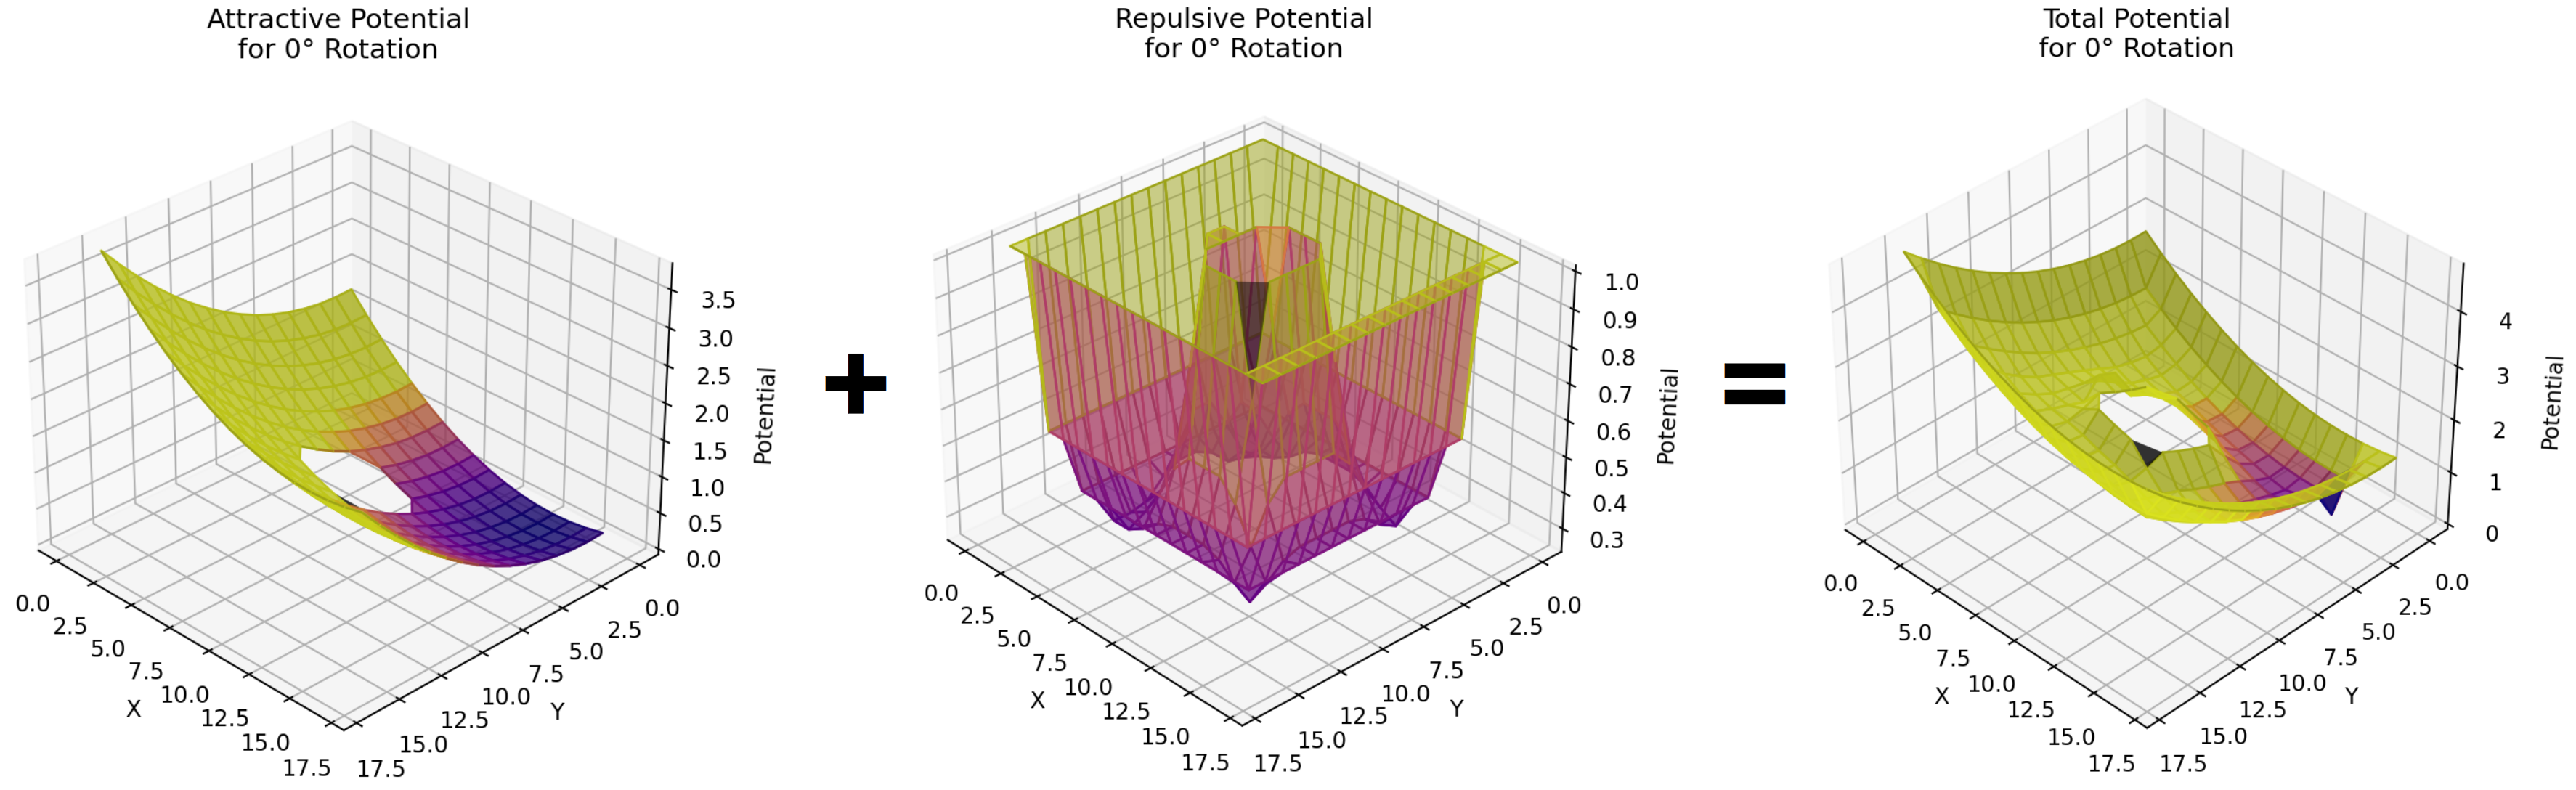
\includegraphics{bilder/total-potential-computation.png}}}
	\caption{Die Berechnung des Gesamtpotenzials für die $0$°-Rotationsebene des Konfigurationsraums mit \texttt{attraction\_weight=5} und \texttt{repulsion\_weight=0}}
\end{figure}

\vspace*{0.2cm}
\section{Wavefront Potenziale}

Choset stellt eine Potenzialfunktion unter Verwendung der Breitensuche ausgehend vom Zielpunkt vor. Beim sogenannten \textit{Wavefront-Algorithmus} entsprechen die Koordinaten des Konfigurationsraums den Knoten der Breitensuche. Jeder besuchte Knoten erhält dabei ein Potenzial, das mit jeder Ebene der Breitensuche streng monoton ansteigt: \cite{choset.2007}
\vspace*{0.1cm}
\begin{algorithm}
\caption{Wavefront-Algorithmus}
	\begin{algorithmic}[1]
  \State \textbf{Initialisierung:}
  \State \hspace{\algorithmicindent} Jeder Punkt $U(\texttt{x}, \texttt{y}, \texttt{rotation}) = 0$
  \State \hspace{\algorithmicindent} Warteschlange $Q := \{((\texttt{x}_{Ziel}, \texttt{y}_{Ziel}, \texttt{rotation}_{Ziel}), 2)\}$
		\vspace*{0.3cm}
  \While{$Q \neq \emptyset$}
      \State $((\texttt{x}, \texttt{y}, \texttt{rotation}), \texttt{potential}) \gets Q$
      \State $U(\texttt{x}, \texttt{y}, \texttt{rotation}) = \texttt{potential}$
      \State Nachbarn $N := \{(\texttt{x-1}, \texttt{y}, \texttt{rotation}), (\texttt{x+1}, \texttt{y}, \texttt{rotation}), ... (\texttt{x}, \texttt{y}, \texttt{(rotation-1) \% rotations})\}$
      \For{$(\texttt{x}_{Nachbar}, \texttt{y}_{Nachbar}, \texttt{rotation}_{Nachbar}) \gets N$}         
          \If{$0 \leq \texttt{x}_{Nachbar} < \texttt{occupancy\_grid\_width}$ \\
              \hspace*{\algorithmicindent}\hspace*{\algorithmicindent} \textbf{and} $0 \leq \texttt{y}_{Nachbar} < \texttt{occupancy\_grid\_height}$ \\
              \hspace*{\algorithmicindent}\hspace*{\algorithmicindent} \textbf{and} $ \texttt{computational\_space}[\texttt{rotation}_{Nachbar}][\texttt{y}_{Nachbar}][\texttt{x}_{Nachbar}] = \texttt{True}$}
              \State $((\texttt{x}_{Nachbar}, \texttt{y}_{Nachbar}, \texttt{rotation}_{Nachbar}), \texttt{potential + 1}) \rightarrow Q$
          \EndIf
      \EndFor
  \EndWhile
	\end{algorithmic}
\end{algorithm}

\newpage
Demnach breitet sich das ansteigende Potenzial, beginnend am Zielpunkt als Quelle, bildlich als \textit{Wellenfront} im Konfigurationsraum aus. Koordinaten in der Nähe von Hindernissen erhalten dabei auf der entgegengesetzten Seite der Ausbreitungsrichtung höhere Potenziale.

\begin{figure}[H]
	\centering
	\footnotesize
	\centerline{\resizebox{1\linewidth}{!}{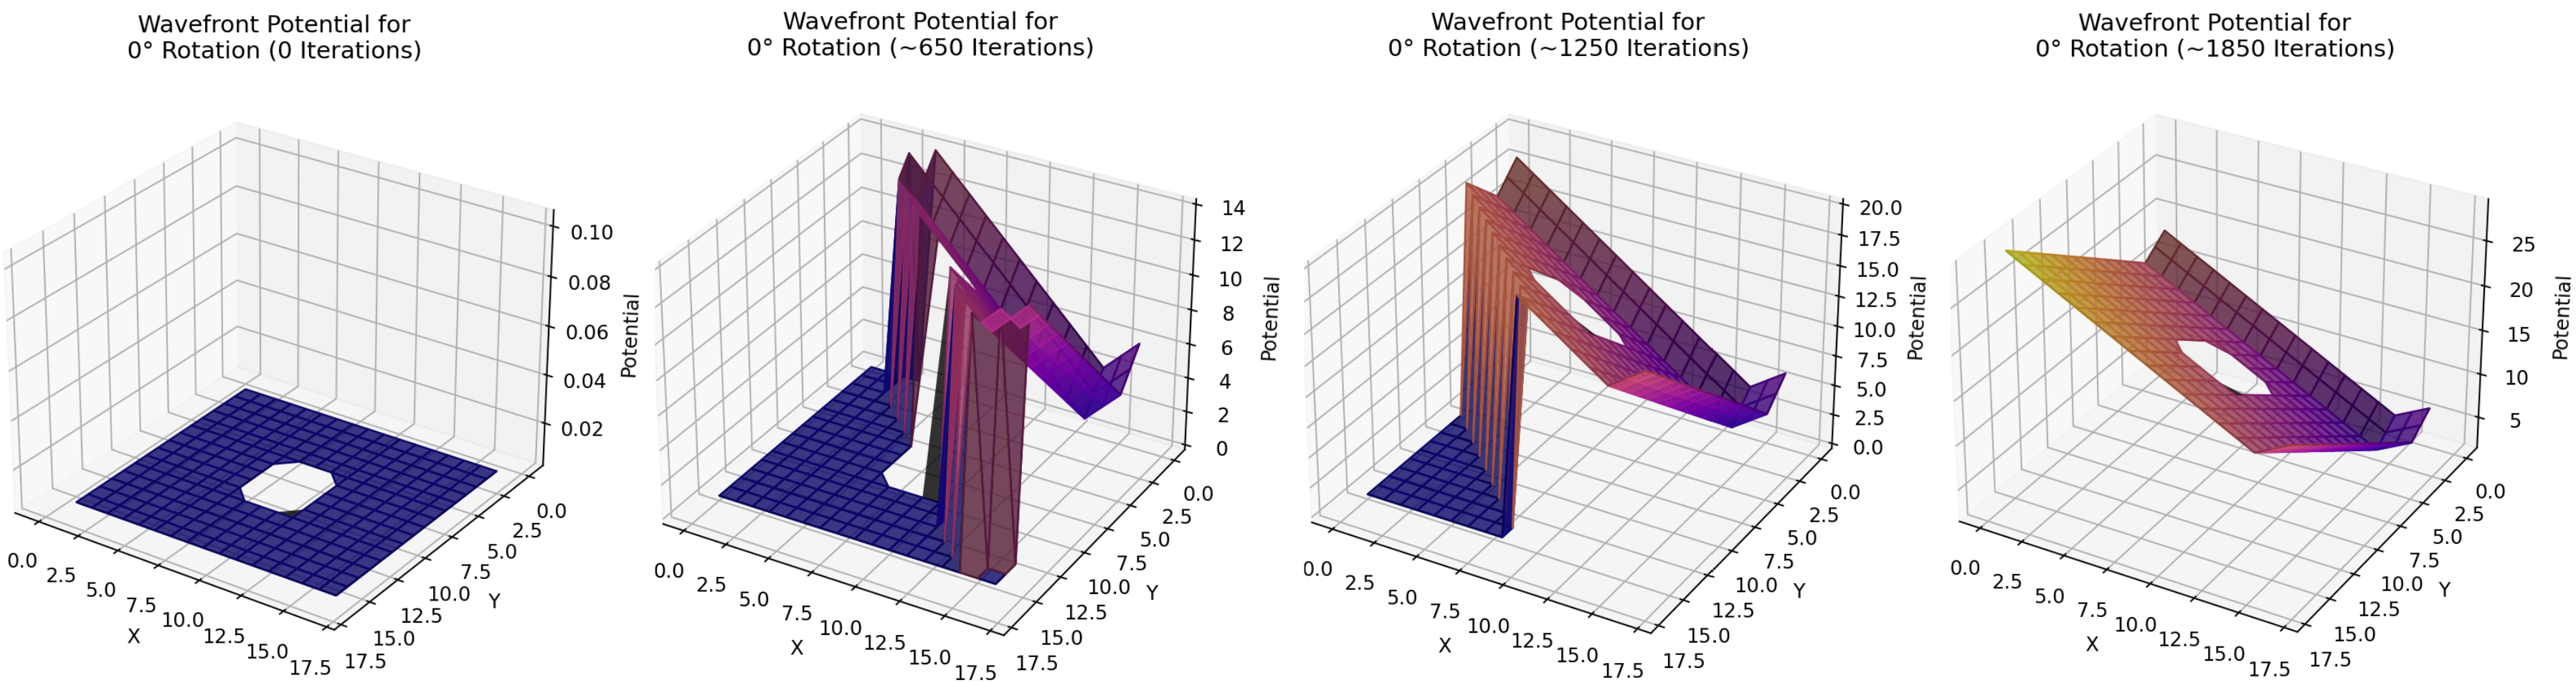
\includegraphics{bilder/wavefront.png}}}
	\caption{Die Berechnung des Gesamtpotenzials für die $0$°-Rotationsebene des Konfigurationsraums mit dem Wavefront-Algorithmus}
\end{figure}

\vspace*{1cm}
Unabhängig von der gewählten Potenzialfunktion wird das Potenzialfeld im dreidimensionalen Konfigurationsraum für jede Rotationsebene berechnet.
Dadurch hat das Potenzialfeld die gleichen Dimensionen wie der Konfigurationsraum:

\begin{figure}[H]
	\centering
	\footnotesize
	\centerline{\resizebox{1\linewidth}{!}{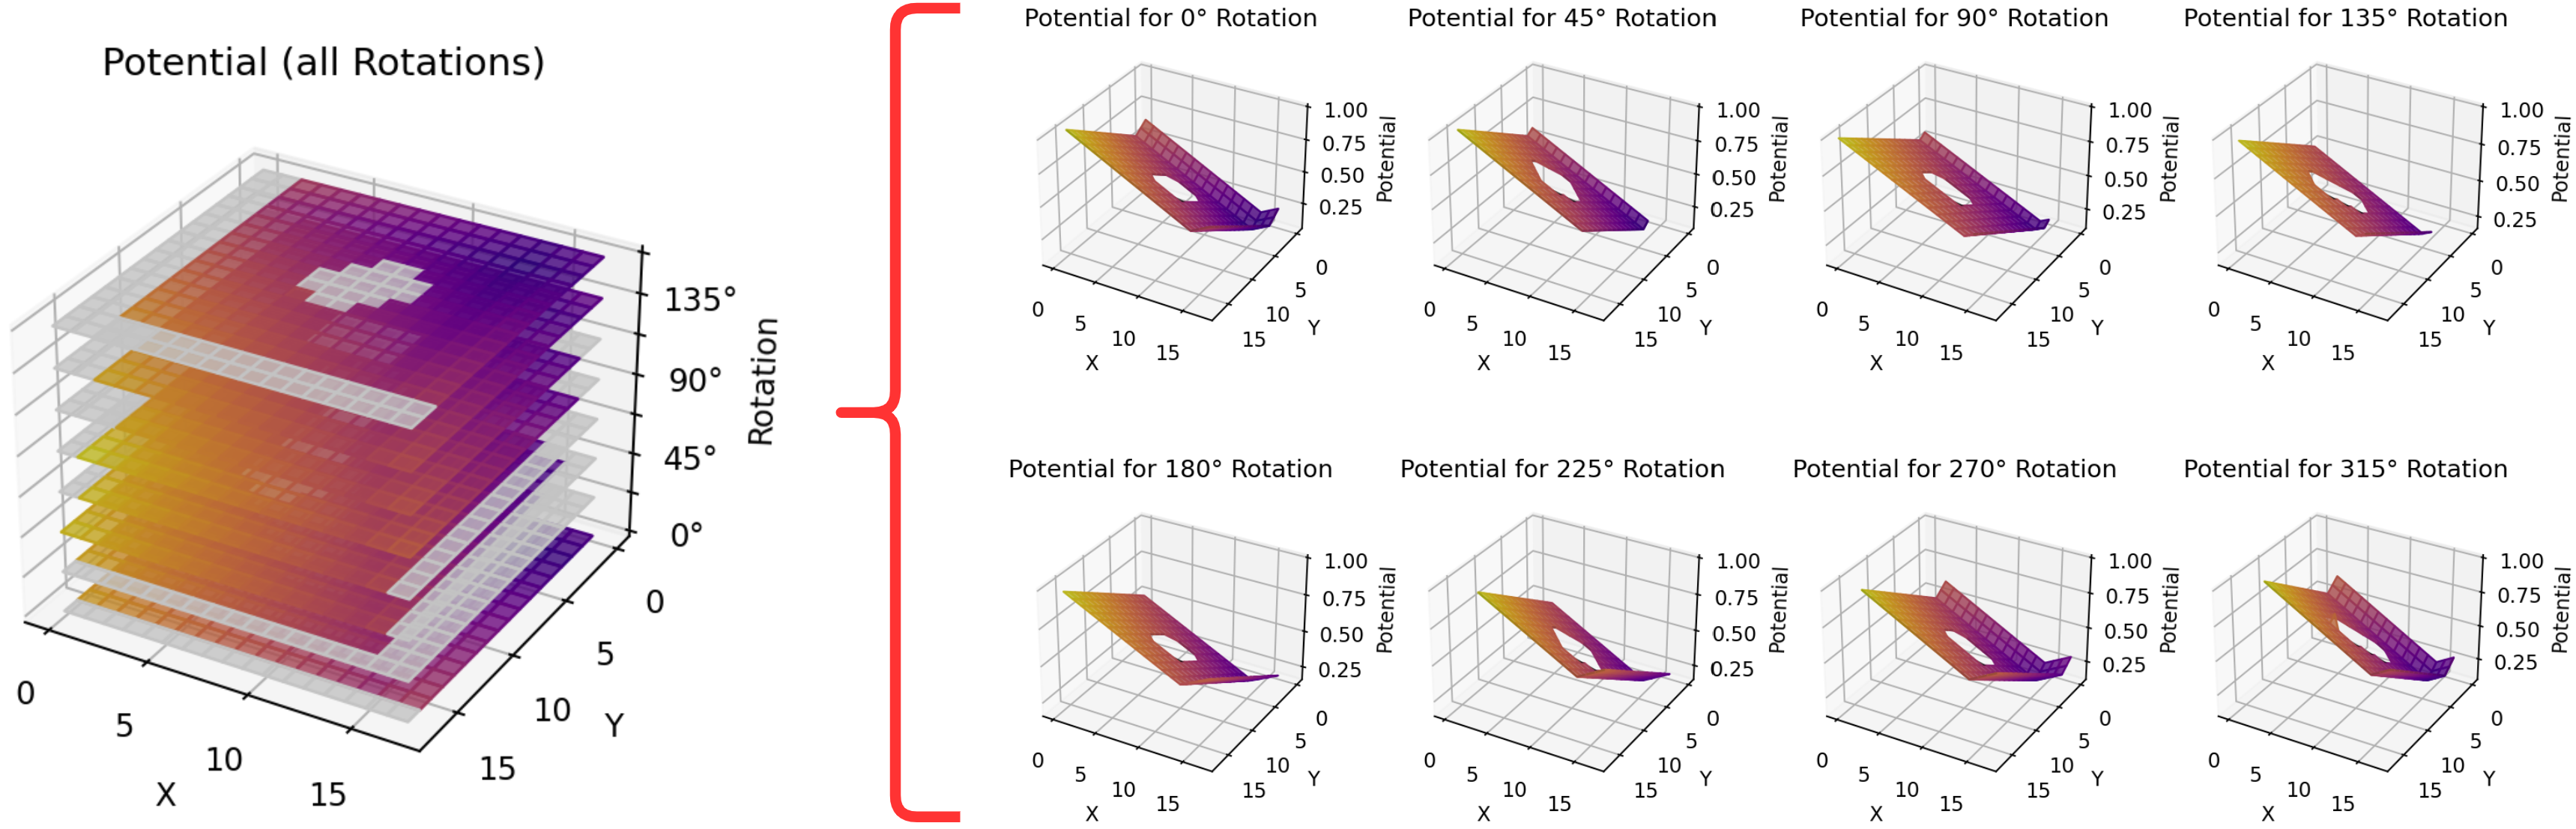
\includegraphics{bilder/potential-stacked-computed.png}}}
	\caption{Das Potenzialfeld wird im dreidimensionalen Konfigurationsraum berechnet.}
\end{figure}




  \chapter{Roboternavigation im Kraftfeld}
\vspace*{-0.2cm}
Die Roboternavigation basierend auf der Potenzialfeldmethode entspricht der Bewegung eines Körpers im \textit{Kraftfeld} des Potenzialfelds.

\vspace*{-0.1cm}
\section{Berechnung der Gradienten}
\enlargethispage{0.9cm}

Das Kraftfeld entspricht dem negativen Gradientenfeld des Potenzialfelds \cite{khatib.1985}. Auf jede Koordinate wirkt eine Kraft $F_{x/y/rotation}(\texttt{x}, \texttt{y}, \texttt{rotation})$ in Höhe der negativen Potentialänderung, zerlegt in die drei kartesischen Komponenten des Konfigurationsraums:
\vspace*{0.13cm}
\begin{equation*}
 F_{x}(\texttt{x}, \texttt{y}, \texttt{rotation}), F_{y}(\texttt{x}, \texttt{y}, \texttt{rotation}), F_{rotation}(\texttt{x}, \texttt{y}, \texttt{rotation}) = -\nabla U(\texttt{x}, \texttt{y}, \texttt{rotation})
\end{equation*}

Um die Gradienten zwischen dem letzten Rotationszustand und $0$° zu berechnen, wird die erste und letzte Rotationsebene an das jeweils andere Ende der Dimension \texttt{potential[rotation]} kopiert:
\vspace*{0.15cm}
\begin{equation*}
\hspace*{-0.0075\linewidth}
\resizebox{1.05\linewidth}{!}{
$
	\texttt{potential\_padded} = \texttt{np.concatenate([potential[rotations-1], potential, potential[0]])}
$
}
\hspace*{-0.0075\linewidth}
\end{equation*}


Die kopierten Rotationsebenen werden nach Berechnung der Kraftfelder entfernt:
\vspace*{0.13cm}
\begin{equation*}
\hspace*{-0.1\linewidth}
\resizebox{1.2\linewidth}{!}{
$
\texttt{force\_field\_rotation}, \texttt{ force\_field\_y}, \texttt{ force\_field\_x} = -\texttt{np.gradients(potential\_padded)[1 : rotations-1]}
$
}
\hspace*{-0.1\linewidth}
\end{equation*}

Somit entspricht $\texttt{force\_field\_rotation[rotations-1]} > 0 $ einer Kraft in Richtung $\texttt{force\_field\_rotation[0]}$ und $ \texttt{force\_field\_rotation[0]} < 0 $ entspricht einer Kraft in Richtung $\texttt{force\_field\_rotation[rotations-1]}$.
\begin{figure}[H]
	\centering
	\footnotesize
	\centerline{\resizebox{0.63\linewidth}{!}{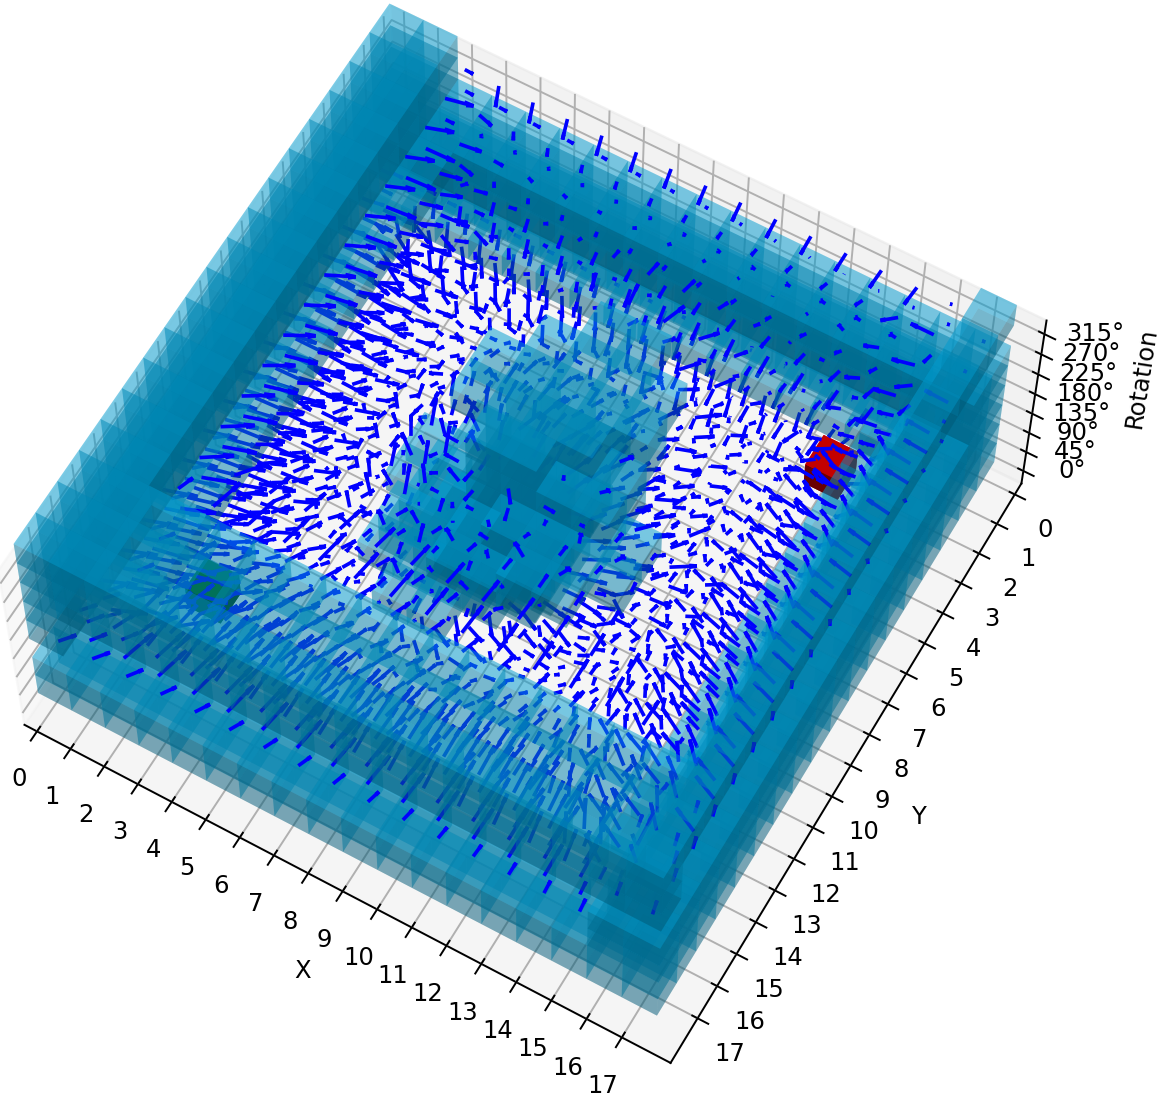
\includegraphics{bilder/force-field.png}}}
	\vspace*{-0.23cm}
	\caption{Darstellung des negativen Gradientenfelds als Kraftpfeile im Konfigurationsraum.}
\end{figure}

\subsection{Gradienten an Grenzen und Hindernissen}

Um die Grenzen des Konfigurationsraums einzuhalten, werden unzulässige Kräfte an den X- und Y-Grenzen auf $0$ gesetzt. Durch dieses manuelle Abschneiden der Kräfte können an den Grenzen lokale Minima entstehen.
\begin{figure}[H]
	\centering
	\footnotesize
	\centerline{\resizebox{0.65\linewidth}{!}{\input{bilder/gradient-clipping_latex.pdf_tex}}}
	\caption{Das Setzen der Gradienten in Grenznähe auf $0$ kann zu lokalen Minima führen.}
\end{figure}
\vspace*{-0.1cm}
Im Numpy Potenzialfeld \texttt{potential} haben Hindernisse das Potenzial \texttt{np.nan}. Somit berechnet \texttt{np.gradients()} für jede an ein Hindernis grenzende Koordinate den Gradienten \texttt{np.nan}.
Um die Kräfte an Hindernissen analog zu Kräften an den Grenzen des Konfigurationsraums zu interpretieren, müssen diese manuell berechnet werden. 
Sollte die berechnete Kraft einer Dimension in Richtung des Hindernisses zeigen, wird diese ebenfalls auf $0$ gesetzt. Nachfolgende Tabelle zeigt dies beispielhaft für Hindernisse im Kraftfeld der X-Achse \texttt{force\_field\_x}:
\begin{table}[H]
\centerline{\resizebox{0.9\linewidth}{!}{
\begin{tabular}{|c|c|c|}
\hline
\textbf{Koordinate Hindernis}                                                & \textbf{\texttt{force\_field\_x[rotation][y][x] = -1*...}}                                                        & \textbf{\texttt{= 0}, wenn ...} \\ \hline
$x+1$ (rechts)                                                               & \texttt{potential[z, y, x] - potential[z, y, x-1]} & $<0$                               \\ \hline
$x-1$ (links)                                                                & \texttt{potential[z, y, x+1] - potential[z, y, x]} & $>0$                                \\ \hline
\begin{tabular}[c]{@{}c@{}}$x+1$ und $x-1$\\ (rechts und links)\end{tabular} & \texttt{0}                                                                           & N/A                                 \\ \hline
\end{tabular}}}
\end{table}
Wird die Kraft einer Dimension auf $0$ gesetzt, wobei die Kräfte der anderen Kraftfelder an dieser Koordinate ebenfalls $0$ sind, entsteht ein lokales Minimum oder Plateau.

\subsection{Behandlung lokaler Maxima}

Im Unterschied zu einem lokalen Minimum oder Plateau ist bei einem lokalen Maximum das Potenzial der Nachbarn streng monoton niedriger als das der aktuellen Koordinate.
In diesen Fällen wird zu einem der beiden Nachbarn ein künstliches Hindernis gesetzt und der Gradient neu berechnet.
\begin{figure}[H]
	\centering
	\footnotesize
	\centerline{\resizebox{0.9\linewidth}{!}{\input{bilder/local-maxima_latex.pdf_tex}}}
	\caption{Lokale Maxima können durch künstliche Hindernisse behoben werden.}
\end{figure}


\section{Gradientenabstieg}

Die berechneten Gradientenfelder ermöglichen die Roboternavigation mit dem \textit{Gradientenabstiegsverfahren}. Pro Verarbeitungsschritt wird die nächste Koordinate basierend auf der betragsmäßig größten Kraft in $F_{x}(\texttt{x}, \texttt{y}, \texttt{rotation})$, $F_{y}(\texttt{x}, \texttt{y}, \texttt{rotation})$ und $F_{rotation}(\texttt{x}, \texttt{y}, \texttt{rotation})$ gewählt, bis eine bereits besuchte Koordinate oder eine Koordinate mit Kräftegleichgewicht $F_{x}(\texttt{x}, \texttt{y}, \texttt{rotation}) = F_{y}(\texttt{x}, \texttt{y}, \texttt{rotation}) = F_{rotation}(\texttt{x}, \texttt{y}, \texttt{rotation}) = 0$ erreicht wird:

\begin{algorithm}
\caption{Gradientenabstiegsverfahren}
\begin{algorithmic}[1]
    \State \textbf{Initialisierung:}
    \State \hspace{\algorithmicindent} $(\texttt{x}_{\text{current}}, \texttt{y}_{\text{current}}, \texttt{rotation}_{\text{current}}) = \texttt{start\_point}$
    \State \hspace{\algorithmicindent} Visited $V \leftarrow \emptyset$
	\vspace*{0.3cm}
    \While{true}
        \If{$(\texttt{x}_{\text{current}}, \texttt{y}_{\text{current}}, \texttt{rotation}_{\text{current}}) = \texttt{goal\_point}$}
            \State \textbf{return} Ziel gefunden
        \EndIf
		\vspace*{0.1cm}
        \State $\texttt{force\_field\_x/y/rotation}\texttt{[}\texttt{rotation}_{\text{current}}\texttt{][}\texttt{y}_{\text{current}}\texttt{][}\texttt{x}_{\text{current}}\texttt{]} = 0$
        \State $(\texttt{dx}, \texttt{dy}, \texttt{drotation}) \gets \max(|\texttt{force\_field\_x/y/rotation}\texttt{[}\texttt{rotation}_{\text{current}}\texttt{][}\texttt{y}_{\text{current}}\texttt{][}\texttt{x}_{\text{current}}\texttt{]}|)$
		\vspace*{-0.3cm}
        \If{$(\texttt{dx}, \texttt{dy}, \texttt{drotation}) = (0,0,0)$}
            \State \textbf{return} Lokales Minimum oder Plateau
        \EndIf
     	\vspace*{0.1cm}
        \State $(\texttt{x}_{\text{current}}, \texttt{y}_{\text{current}}, \texttt{rotation}_{\text{current}}) \gets (\texttt{x}_{\text{current}} + \texttt{dx}, \texttt{y}_{\text{current}} + \texttt{dy}, \texttt{rotation}_{\text{current}} + \texttt{drotation})$
		\vspace*{-0.3cm}
        \If{$(\texttt{x}_{\text{current}}, \texttt{y}_{\text{current}}, \texttt{rotation}_{\text{current}}) \in V$}
            \State \textbf{return} Lokales Minimum
		\Else
			\State $(\texttt{x}_{\text{current}}, \texttt{y}_{\text{current}}, \texttt{rotation}_{\text{current}}) \rightarrow V$
        \EndIf
    \EndWhile
\end{algorithmic}
\end{algorithm}

Gemäß der in Kapitel \ref{ch:roboterbewegung} definierten Roboterbewegungen darf pro Verarbeitungsschritt nur eine Translation um eine Einheit entlang der Dimensionen des Konfigurationsraums  durchgeführt werden: $ (\texttt{dx}, \texttt{dy}, \texttt{drotation}) \in \{(\texttt{1},\texttt{0},\texttt{0})(\texttt{-1},\texttt{0},\texttt{0}),(\texttt{0},\texttt{1},\texttt{0}),(\texttt{0},\texttt{-1},\texttt{0}),(\texttt{0},\texttt{0},\texttt{1}),(\texttt{0},\texttt{0},\texttt{-1})\}$
\vspace*{0.1cm}
\begin{figure}[h!]
	\centering
	\footnotesize
	\centerline{\resizebox{1\linewidth}{!}{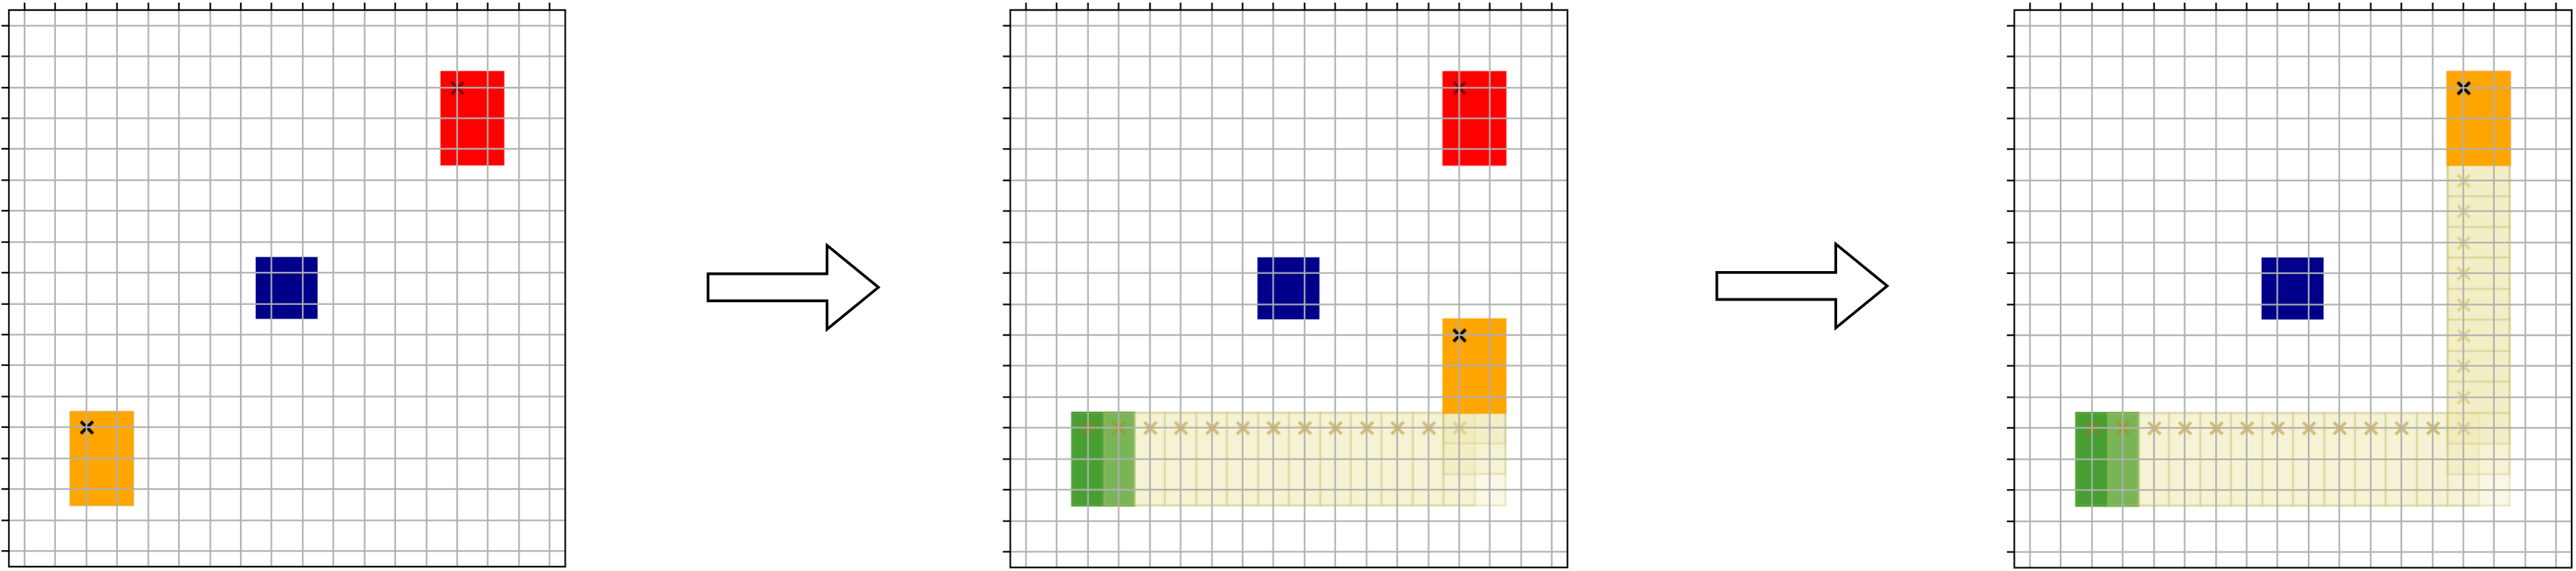
\includegraphics{bilder/grad-desc.png}}}
	\caption{Roboternavigation über das Gradientenabstiegsverfahren im Kraftfeld des Wavefront-Potenzialfelds.}
\end{figure}






  \chapter{Diskussion}

\section{Anziehendes und abstoßendes Potenzial: Lokale Minima und Oszillationen}

Eine Eigenschaft der Potenzialfunktion mit anziehendem und abstoßendem Potenzial ist die Konvergenz des Gradientenabstiegsverfahren zu einem lokalen Minimum bei konkaven Hindernissen.
Davon betroffen sind Occupancy Grids, deren Hindernisse Polygone mit überstumpfen Winkeln ($180\text{°} \le \text{Winkel} \le 360\text{°}$) bilden.
Bekannte Beispiele der Literatur sind C- und U-förmige Polygone \cite{maqbool.2021, yujiang.2017}:
\begin{figure}[h!]
	\centering
	\footnotesize
	\centerline{\resizebox{0.3\linewidth}{!}{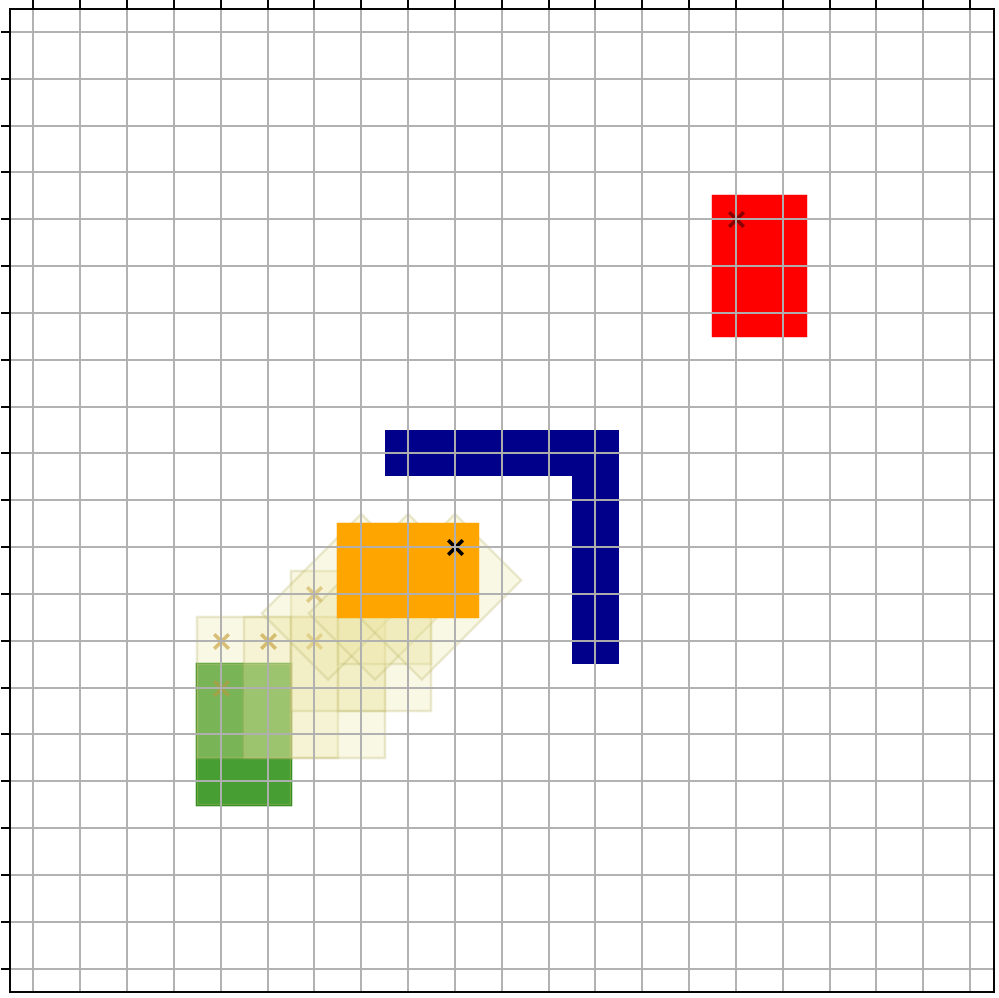
\includegraphics{bilder/attr-repul-c-shape.png}}}
	\caption{Für konkave Hindernisse konvergiert das Gradientenabstiegsverfahren mit anziehendem und abstoßendem Potenzial.}
\end{figure}

Weiterhin führt das Gravitationsfeld von Potenzialfeldern mit anziehendem und abstoßendem Potenzial zwischen Hindernisengstellen zu Oszillationen. Der Roboter wechselt bei dieser Art des lokalen Minimums zwischen zwei Koordinaten mit entgegen gerichteten Gradienten.
Insbesondere kleine Occupancy Grids sind von diesem Effekt betroffen, da die Grenzen des Potenzialfelds als Hindernisse berücksichtigt werden. Abbildung \ref{fig:oscillation} zeigt diesen Effekt Anhand des Potenzialfelds aus Kapitel X (TODO).
Die Erhöhung des Abstandes zwischen Occupancy-Grid-Grenzen und Hindernissen vermeidet dieses Problem.

\begin{figure}[h!]
	\footnotesize
	\centering
	\hspace*{\fill}
	\begin{minipage}{0.46\textwidth}%
		\centerline{\resizebox{0.6\linewidth}{!}{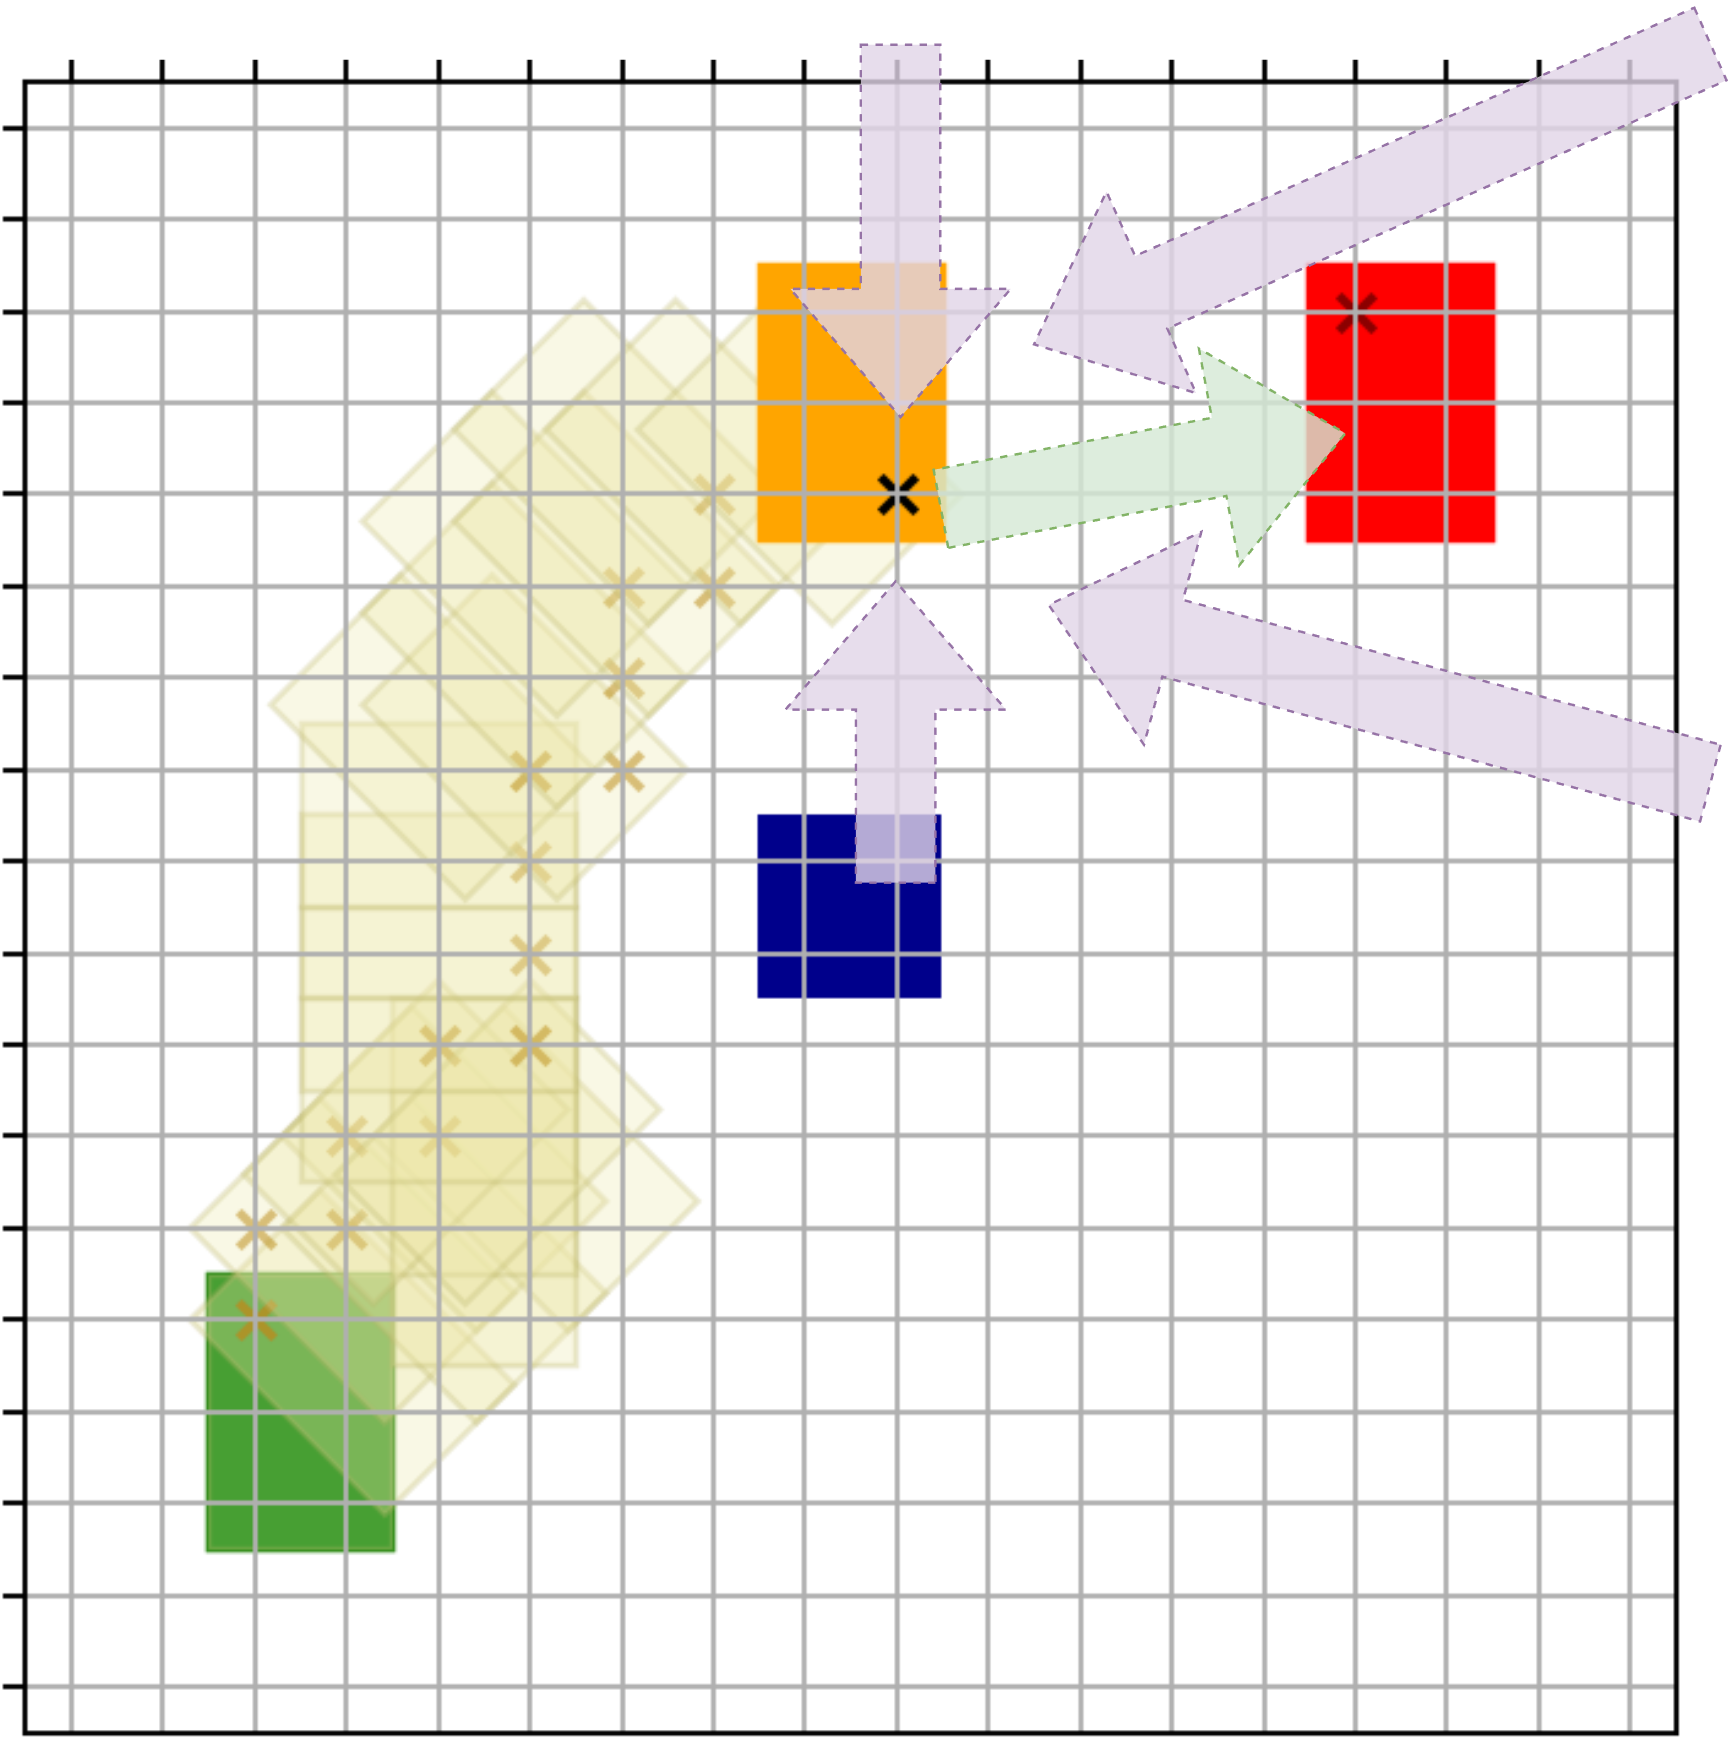
\includegraphics{bilder/attr-repul-oscillating-arrow.png}}}
	\end{minipage}
	\hspace*{\fill}
	\begin{minipage}{0.46\textwidth}%
		\footnotesize
		\centerline{\resizebox{0.6\linewidth}{!}{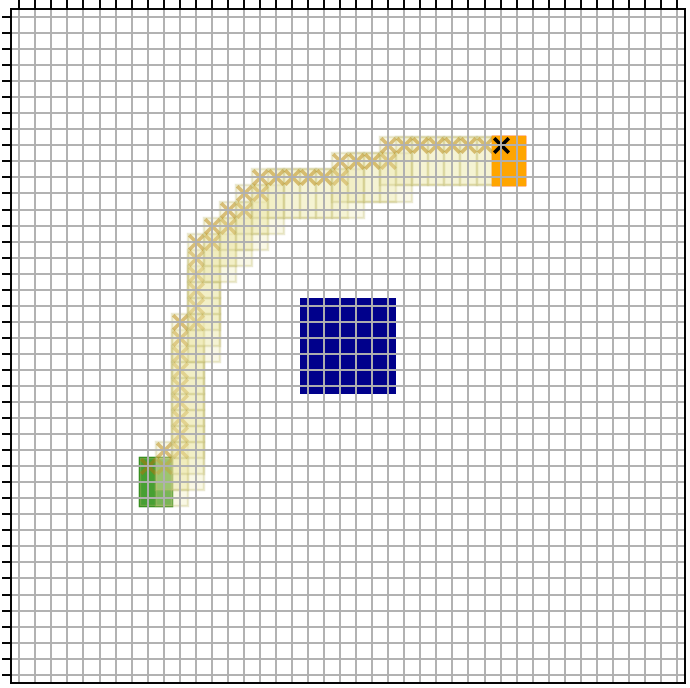
\includegraphics{bilder/attr-repul-oscillating-scaled.png}}}
	\end{minipage}
	\hspace*{\fill}
	%	\vspace{-1cm}
	\label{fig:oscillation}
	\caption{Bei Engstellen heben sich die abstoßenden Kräfte zwischen Hindernissen auf (links), bei hinreichend Abstand nicht (rechts).}
\end{figure}


Im Gegensatz dazu verhindert die streng monotone Potenzialänderung des Wavefront Algorithmus die Konvergenz zu lokalen Minima, sofern sich das Ziel an einem für den Roboter physikalisch erreichbaren Punkt befindet.

	- Konvergiert nie zu lokalem Minima
	- Potenziale nur in physikalisch erreichbaren Regionen definiert

*** TODO: Abbildungen mit unterschiedlichen Wavefront Szenarien ***


\section{Überdeckungen des Robotermodells mit Hindernissen}

Beobachtung bei den getesteten Szenarien der Implementierung: 
- Schlechte Interpolation der rotierten Robotermaske für kleine Roboterdimensionen mit kleinen Rotationsschritten in einem kleinen Occupancy Grids
 *** TODO: Beispiel Interpolation für 1x3 bei 10° ***

In Literatur (Author Wavefront) deshalb empfohlen: mit kleinen Rotationsschritten die Roboterdimensionen und das Occupancy Grid zu skalieren
=> Erhöht die Auflösung der Robotermaske, verringert Artefakte der Interpolation

*** TODO Beispiel Skalierung ***

  % Literatur anzeigen
  \printbibliography
  
\end{document}